\documentclass{bioinfo}
\copyrightyear{2015}
\pubyear{2015}

%%% SETTINGS %%%
\usepackage{tikz} %ticks in tables
\def\checkmark{\tikz\fill[scale=0.3](0,.35) -- (.25,0) -- (1,.7) -- (.25,.15) -- cycle;}
\usepackage{listings} %code format
\usepackage{color}
\definecolor{lightgray}{rgb}{.9,.9,.9}
\definecolor{darkgray}{rgb}{.4,.4,.4}
\definecolor{purple}{rgb}{0.65, 0.12, 0.82}
\definecolor{darkgreen}{rgb}{0.0, 0.2, 0.0}

\lstdefinelanguage{JavaScript}{
  keywords={break, case, catch, continue, debugger, default, delete, do, else, false, finally, for, function, if, in, instanceof, new, null, return, switch, this, throw, true, try, typeof, var, void, while, with, attr, text, select},
  morecomment=[l]{//},
  morecomment=[s]{/*}{*/},
  morestring=[b]',
  morestring=[b]",
  ndkeywords={class, export, boolean, throw, implements, import, this, D3, append},
  keywordstyle=\color{blue}\bfseries,
  ndkeywordstyle=\color{red}\bfseries,
  identifierstyle=\color{black},
  commentstyle=\color{purple}, %commentstyle=\color{purple}\ttfamily,
  stringstyle=\color{darkgreen}, %stringstyle=\color{darkgreen}\ttfamily,
  sensitive=true
}

\lstset{
   language=JavaScript,
   backgroundcolor=\color{lightgray},
   frame=single,
   extendedchars=true,
   basicstyle=\footnotesize\ttfamily,
   showstringspaces=false,
   showspaces=false,
   numbers=left,
   numberstyle=\footnotesize, % numberstyle=\footnotesize\color{lightgray},
   numbersep=5pt,
   tabsize=2,
   breaklines=true,
   showtabs=false,
   captionpos=b
}


%%% DOCUMENT %%%
\begin{document}
\firstpage{1}

\title[short Title]{Data visualization using D3}
\author[Data visualization using D3]{Jes\'us Alejandro Vald\'es Vald\'es, and Philipp M\"uller}
\address{}
\history{}
\editor{}

\maketitle

\begin{abstract}
\section{Motivation}
\hfill \break
Long before people started to collect data in a digital format, they depended on visual representations of data such as maps.

One of the earliest devices to visualize the abstract concepts of the numerical system and basic arithmatics was the Abacus. %\citep{wiki:abacus}.
Numbers are represented by balls on a wire, shifting them from left to right you can add or subtract values and count the remaining balls \ref{fig:abacus}.
This simple visualization of the numerical system and basic arithmatics is still used today in pre-schools and elementary schools, because visualizations convey information in a universal manner and make it simple to share ideas with others.
\newline
As huge amounts of data are collected data visualization software becomes more in more important. A visual representation enables us to find relevance of millions of variables, communicate concepts and even predict future behaviour based on patterns.
\newline
On this and the following pages we will discuss different visualization methods for data in a web based context, available Java Script libraries, why we decided to use D3.js and it's core concepts.
\begin{figure}[!tpb]
\centerline{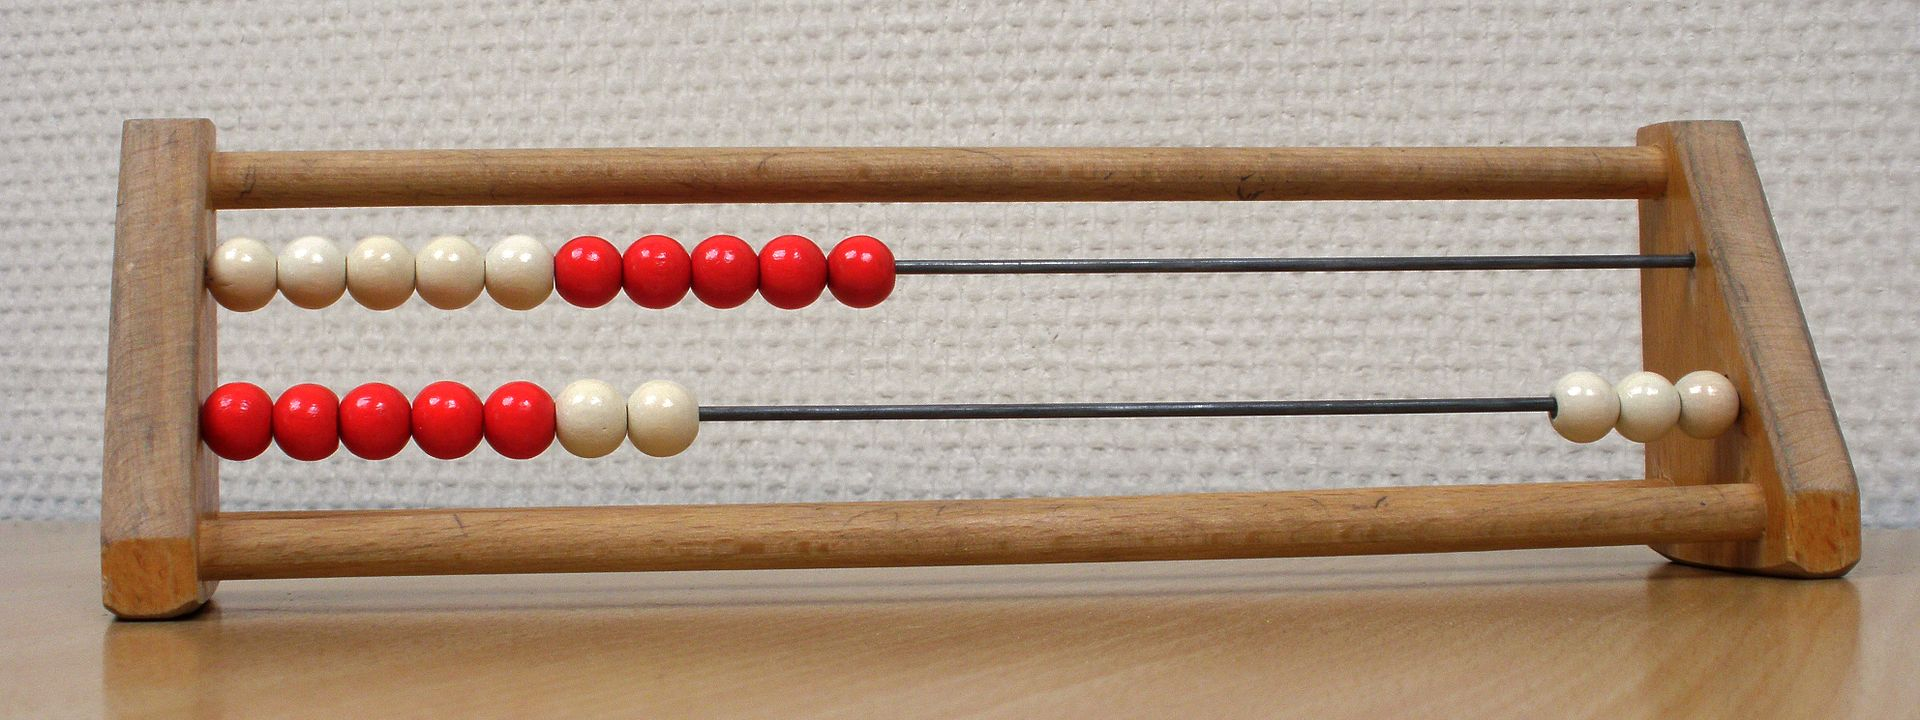
\includegraphics[width=70mm]{abacus.jpg}}
\caption{Simple abacus}\label{fig:abacus}
\end{figure}

\section{Availability}
\hfill \break
D3.js is a free Java Script library which can also be customized according to your own needs.

\section{Contacts}
\hfill \break
Jes\'us Alejandro Vald\'es Vald\'es: alejandro.valdesval@gmail.com \newline
Philipp M\"uller: philipp.mueller@tum.de
\end{abstract}

\section{Introduction}
\subsection{How can we visualize data in a browser}
Before we move on what libraries exist to represent data in web browsers we first have to talk about the different approaches how we can draw in our browser in general.
\newline
There exist three main approaches to draw data in modern web browsers, namly:
\begin{enumerate}
\item HTML elements
\item Canvas
\item SVG
\end{enumerate}

% HMTL ELEMENTS
\textbf{HMTL elements} can be styled to represent data, for example a div could be used with different width, height and color parameters to represent a bar in a bar chart.
However building a framework solely on HTML elements and styling them is clunky and does not scale well.
The reason why it doesn't scale well is that complex or round shapes are hard to do with HTML elements and come with performance issues. The performance issues are the result of hundreds or tousands pixel small HMTL elements you need to create and draw to be able to represent complex shapes.
HTML elements are supported in every browser.
They also provide the same functionalities as DOM elements like mouse events and other behaviour, because they are basically just DOM elements.
Another advantage of DOM elements is that they can be styled with CSS (Cascading Style Sheet) files.

\hfill \break
% CANVAS
\textbf{Canvas} is a HMTL5 element and can be seen as a scriptable Bitmap drawing surface.
It provides different drawing methods that enable us to visualize every shape we want to.
Canvas however doesn't have any knowledge about the drawn objects, it only draws pixels.
This also means that there are no predefined event callbacks per element that we are used to from DOM elements.
Another feature of Canvas that might be problematic is that Canvas redraws the visualization with a fixed update rate. This might put unnecessary strain on your computational ressources.
The support for Canvas for the main browsers can be found in table \ref{t:support}, where the lowest browser version is listed to support all features.

% SVG
\textbf{SVG} is also a HTML5 element and defines a sciptable drawing surface. SVG stands for Scaleable Vector Graphic, which implies that it is resolution independent. Resolution independence means in this case that, independent of your zoom level, round shapes stay round and don't get pixelated. 
It also provides many drawable elements that can be modified by parameters to visualize every shape we want to. Different to Canvas SVG elements are DOM elements, this means we can easily define event callbacks on them. SVG also provides simple functions to animate elements.
The support for SVG for the main browsers can also be found in table \ref{t:support}.

\begin{table}
\begin{tabular}{ l | c | c | c | c | c } 
		& Chrome & Internet Explorer & Firefox & Safari & Opera \\
\hline
Canvas	& 4.0 & 9.0 & 2.0 &	3.1 & 9.0 \\
SVG		& 4.0 & 9.0 & 3.0 &	3.2 & 10.1 \\
\end{tabular}
\caption{Support table for HTML5 elements Canvas and SVG} \label{t:support}
\end{table}

In comparison Canvas is performancewise faster than SVG if very many objects have to be drawn.
For our project however we decided to use SVG over Canvas, because we wanted to create a interactive data visualization with not that many objects. On SVG it is very easy to define callback functions for different events such as mouse click and therefore helps us to create a more interactive web application.

\subsection{Data visualization libraries}
There are a huge amount of data visualization libraries available online.
Therefore we had to select a few libraries of this huge amount. 
Our criteria were the size of the community, the support and the documentation, because we had to learn everything from the start.
The following table \ref{t:libs} shows a small selection which mostly or complete satisfied our criteria.

\begin{table}
\begin{tabular}{ l | c | c | c }
Library 			& SVG			& Canvas 		& HTML elements \\
\hline
D3.js				& \checkmark 	& \checkmark 	& \checkmark 	\\
Raph\"ael.js		& \checkmark 	& \textbf{-}	& \textbf{-}	\\
vis.js 				& \checkmark 	& \checkmark 	& \checkmark 	\\
Paper.js			& \textbf{-}	& \checkmark 	& \textbf{-}	\\
Chart.js			& \textbf{-}	& \checkmark 	& \textbf{-}	\\
and many more 		& \vdots 		& \vdots 		& \vdots 		\\
%\hline  
\end{tabular}
\caption{Small selection of available JavaScript data visualization libraries and their base method} \label{t:libs}
\end{table}

% D3.JS
\hfill \break
To note here is that D3.js is a general purpose visualization JavaScript library. It is used for manipulating documents based on data without being coupling with a proprietary framework.
That simply means that you don't have to learn a new visualization language or syntax if you already know SVG or Canvas.
\newline
% RAPHAEL.JS
The Raph\"ael.js library uses the SVG WC3 recommendation and VML (Vector Markup Language) to create graphics. This enables Raph\"ael to be compatible with older browsers as well as modern browers.
\newline
The vis.js library uses different visualization methods, depending on the wanted graph / representation.
\newline
% CHART.JS
The Chart.js JavaScript library uses the HTML5 canvas element but also provides polyfills in order to support older browers like IE7/8.
\newline
% PAPER.JS
The Paper.js library uses the HTML5 Canvas element to draw the data.
\newline
\hfill \break
In our application we decided to use D3.js, because it has a good, active and big community as well as a very good documentation with many great examples.
If this wouldn't be enough you can also find many well written tutorials which helped us to understand D3.
Another important criteria in our case was time. D3 in conjunction with SVG it is very easy and fast to develope a nice looking interactive web application.
\newline
\hfill \break
% WHY D3?
We chose D3 over all other libraries because of its good documentation and exellent tutorials.
D3 also was easy to use with SVG, because SVG elements are DOM elements and D3 uses DOM to bind data, more on that in the following section \ref{s:d3}.



\section{D3 - Data Driven Documents} \label{s:d3}
A brief history of D3
As we have mentioned before, one of the most important libraries for visualization and the main topic of this paper is the JavaScript library D3, D3 stands for Data Driven Documents and its main function is to bind data to the DOM with the goal of creating stunning interactive data oriented visualizations suitable for the web, to do this it uses SVG (scalable vector graphics) elements. D3 was developed in the year 2011 mainly by Mike Bostock and Jeffrey Heer, which were also the main developers for D3’s processor Protovis.
\newline
\hfill \break
Protovis was developed in the year 2009 amid a growing necessity of new technologies capable of creating visual content for the web, the strongest points of Protovis were that it was a Plugin-less library, it didn’t need a plugin to work while most of the other visualization libraries strictly needed one to work, it was also designed to be accessible to non-programmers as it was a learn by example library.

\subsection{Loading of external data}
The Data in D3
It was previously stated that D3 stood for Data Driven Documents, but what exactly is data and how can a developer obtain it? The easiest way of representing data using JavaScript is through the use of a variable, of course a developer can also opt for more powerful data structures, such as an array, a matrix or even objects and arrays of objects, this could empower the developer to create simple static data visualizations, or visualizations made using user input. A way more useful way of using data in D3 is importing it from a file or through an API call, and D3 gives us methods to do this. 
Using for example the csv, html, json, tsv, xml or xhr methods a developer could obtain data from different sources.

\subsection{Selections}
Of course after a developer has found suitable data for his work, he now needs a way of binding said data to a DOM element so that it can be visualized in a web site. D3 has the ability to do so, with its select() and selectAll() methods. These methods will return an array of elements from the current document.
Selections in D3 use CSS3 to select elements which means that you can select DOM elements the following ways:
\begin{itemize}
\item Tag ("div")
\item Class (".myClass")
\item Id ("\#thisID")
\item Attributes ("[color=red]")
\item Logical AND (".this.that")
\item Logical OR (".this, .that")
\end{itemize}
Once a selection is retrieved, operators can be applied to it to modify it on many ways, for example, set or get attributes, styles, properties, HTML and text content. Probably the most powerful thing to do with a selection is to join it to a data set (this will be described in more depth on the next section).
Thanks to this approach, that allows us to operate on entire selections at once, the use of for loops is rarely needed. D3 also allows method chaining on its selections which makes code more readable and understandable, this looks like the next piece of code:
\begin{lstlisting}
D3.select("body")
	.append("div")
	.attr("class","divClass")
	.append("p")
		.text("I am a paragraph")
		.attr("class","pClass");
\end{lstlisting}
This code snippet only selects our body element then it adds a div element to it, as from this moment on the following methods will act on the new dix element, so the new class name will be for our div not our body element, then inside the div it´ll add a p element, and as before the following methods will affect our new p element, this happens because the append method return a new selection, when no selection is returned it will return the last working selection.

\subsection{Joins}
D3s main goal is to visualize data. Since we already know how one can obtain data and how one can select certain DOM elements using D3, the concept of data join can now be discussed. Joins are basically what makes D3 so powerfull and allows it to visualize data, using the \textit{.data([values[, key]])} method.
This method joins data specified in values with the selection the method is called upon, it returns again a selection.
The value parameter can either be specified as an array containing any kind of homogeneous information or a function that returns an array.
The key parameter is optional and specifies a custom compare callback function.
This function will be used to compare and join selection elements and data elements.
If no function is defined as key parameter D3 will revert to the default function that joins selection elements and data based on their indices.

\subsection{The Update, Enter, and Exit sub selections}
When we join data on a selection D3 provides us with three different sub selections as seen in figure \ref{fig:venn}.
These sub selections can be defined as:
\begin{enumerate}
\item The \textbf{update} sub selection is obtained by calling the \textit{.data(values)} operator on a selection. This operator will also save the other two sub selections as references and return them in the update sub selection.
The update sub selection contains all elements for which there exists corresponding data.
\begin{lstlisting}
var updateSubSelection = d3.select("svg").selectAll("rect").data([values]);
\end{lstlisting}
In this example we join our data values on a selection which contains all rectangles in the first svg element we find in our current document.

\item The \textbf{enter} sub selection can be accessed by calling the operator \textit{.enter()} on the update sub selection.
The enter sub selection contains all data values that did not find a partner in our currently displayed selection of elements. We can initialize the data sub selection by appending to it. Otherwise changes to the sub selection won't persist.
\begin{lstlisting}
var enterSubSelection = updateSubSelection.enter().append("rect");
\end{lstlisting}
As mentioned before, in order to add the data to our document we have to add DOM elements containing our data into to document. In this example we used the append method to do so.
Interesting to node here is that after calling the append operator the variable updateSubSelection will also contain our newly added elements that are also in our enterSubSelection.
Therefore we must be careful in what order we call our operators on the update and enter sub selections.

\item The exit sub selection can be accessed by calling the operator \textit{.exit()} on the update sub selection.
The exit sub selection contains all elements of the selection that did not find a partner in the data values.
Often we want to remove those elements from the document. This can be done via \textit{.remove()} call on the exit sub selection as shown in the following example:
\begin{lstlisting}
var exitSubSelection = selection.exit();
exitSubSelection.remove();
\end{lstlisting}
\end{enumerate}

This seperation of the join into three disjunktive sets allows us to specify precisely what operations have to run on which elements. Due to its disjunktive natur this can also improve the performance because we don't have to handle all sub selections, but pick the sub selections we are interested in.
Which brings us back to the meaning of D3, Data Driven Documents.
As we have seen we can transform documents based on data, e.g. the creation and destruction of DOM elements by calling operators on sub selections, which we obtain via data joins on selections.
We can also modify them by calling different available operators such as .attr(), .style() and .text() on selections.
Changes in those selections can be animated via the .transition() operator that we will discuss in the section \ref{s:transitions}.

\begin{figure}[!tpb]
\centerline{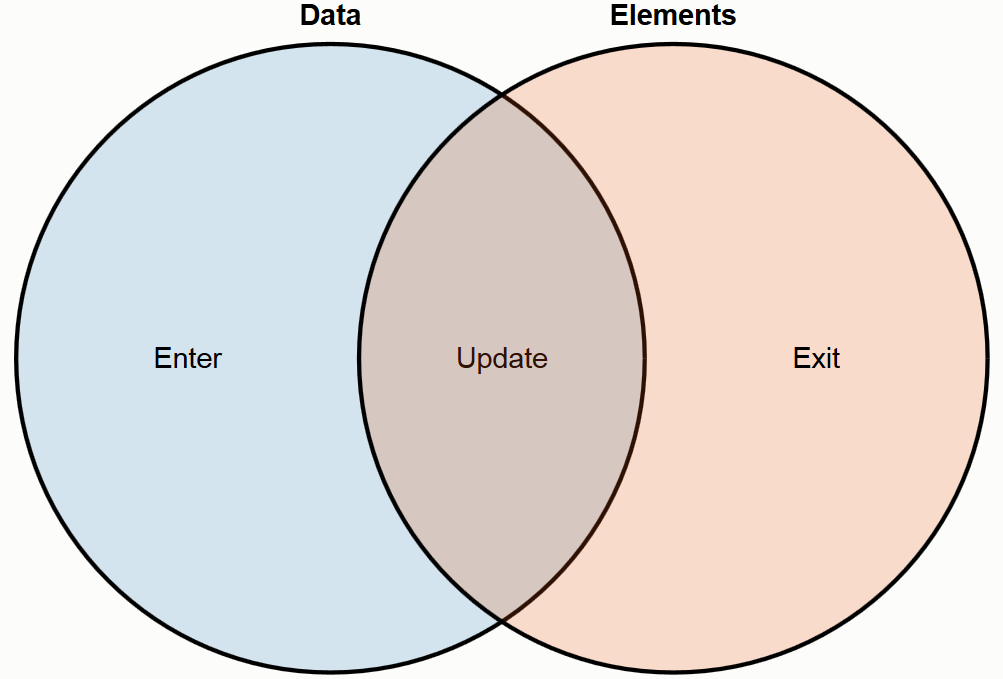
\includegraphics[width=70mm]{vennDiagram.PNG}} %TODO reference to mike bostocks blog
\caption{Venn diagram}\label{fig:venn}
\end{figure}


\subsection{Dynamic properties}
As mentioned in the section before D3 enables us to modify selections dynamically.
The syntax has many similarities with jQuery, however there exists a big difference.
Properties such as stlyles, attributes and text can not only be specified as a constant but also as a function of data and the index associated with the element that calls the method.
To better understand this concept the following example shows how we can use dynamic properties.
The following code shows how we could set the name and font size of each paragraph to a constant variable.
We assume we only have three paragraphs in our HTML body.
\begin{lstlisting}
d3.select("body").selectAll("p")
    .text("See")
    .style("font-size", "8px");
\end{lstlisting}
This however might not be want we want. 
If we want to set the name of each paragraph to a different value and also increase the font size with increasing indice of the paragraph, the code could look something like this:
\begin{lstlisting}
d3.select("body").selectAll("p")
    .data(["See", "The", "World"])
    .text(function(d) { return d; })
    .style("font-size", function(d,i) { return (i*4+8) + "px"; });
\end{lstlisting}
Here we join the selection with data values which represents our paragraph names. Further we call our text and style operators on the update sub selection that will contain all three p-elements, because we join based on array indices.
As you can see the operators have a function defined in them. If you define a function D3 will pass this function the self reference of the element (this), the associated data value as first parameter and the global index of the element in the array as second parameter. Both parameters are optional. 
Based on those informations we define for example the font size in the style property by the base value of 8 pixels plus four times the index of the element.


\subsection{Transitions} \label{s:transitions}
It has been described how a developer could select an element and change its attributes, however these changes would take place immediately, luckily D3 provides the ability to apply these exacts changes over time, thus achieving an animation effect, the transitions have the following life cycle:
\begin{enumerate}
\item The transition is scheduled. (Gets schedule with selection.transition() call in JS)
\item The transition starts. (After the delay, if delay was specified)
\item The transition runs.
\item The transition ends
\end{enumerate}
It is important to notice that transitions are exclusive and only act one given element, so only one transition can be executed at a given time, any new transitions will immediately stop any transitions that were running.

\subsection{Our web application - See the world}
To demonstrate the amazing powers of D3 we developed a small web application that would allow us to get a feeling of what working with D3 really meant. The application is called “See the World” and is meant to be used to create social conscience for the difference between countries. Using an interactive map users can select any country in the world and click on it to see a grahpical representation of data like how many citizens out of 100 have internet access, or the average yearly income per capita.
\newline
All of the visual elements were created with HMTL5 SVG and D3. The data gets pulled from the world bank API, which means an internet connection is needed. To see the source code or simply use the app, got to https://github.com/PhilippMueller1991/JS-Visualization

\subsection{Discussion}
\subsubsection{Disadvantages of D3}
\hfill \break
D3 is a very powerful library however it does have disadvantages for example, it has a steep learning curve and as it is largely used with SVG elements one could say that it is not IE8 compatible, also even though D3 can be used to create charts it’s not a graphing library, the user should not expect really easy out of the box methods that would do all of the work, such as makePieChart(50,50), another big disadvantages is that because it works with the DOM response time can become problem on very large documents.

\subsubsection{Advantages of D3}
\hfill \break
However D3 also has a lot of advantages mainly that it has a great community and that because it is not a graphing nor a charting library it gives the user creative freedom to visualize whatever they want, however they want. Other advantages are that it uses commonly known selectors, the transitions and its fast development cycle.


\section{Conclusion}
Throughout this report we’ve learned about one of the biggest visualization library for JavaScript which in the last couple of years has been used by data visualizers all over the globe to represent data in ways that break past barriers of simple charts and plots.
We´ve learned about the backbone of D3 and how it allows us not only to create static content, but also dynamic real time applications, and that with the help of its great community and documentation, anyone with some previous JavaScript knowledge can start creating his/her own visualizations, that is if they dedicate enough time to go over the steep learning curve.

To finish this report it’s necessary to point out in which cases it’s better to opt for other technologies.

\subsection{When not to use D3}
\hfill \break
\begin{enumerate}
\item No time to learn
\item Advanced big data operations are needed
\item Real graphing software is needed
\end{enumerate}

\subsection{When to use D3}
\hfill \break
\begin{enumerate}
\item Visualization of basically anything
\item Creativity is needed
\item Quick prototyping
\end{enumerate}

\end{document}
